\documentclass[12pt,a4paper, french]{report}

% ================================
%            PACKAGES
% ================================

\usepackage[T1]{fontenc}
\usepackage[utf8]{inputenc}
\usepackage[french,english]{babel}
\usepackage{xcolor}
\usepackage{graphicx}
\usepackage{fancyhdr}
\usepackage{amsmath}
\usepackage{eso-pic}
\usepackage{leftidx}
\usepackage{float}
\usepackage{lastpage}
\usepackage{caption}
\usepackage[colorlinks=true,
            urlcolor=black,
            linkcolor=black,
            breaklinks=true,
            citecolor= black,
            plainpages=false
            ]{hyperref}
            

% ================================
%            SETTINGS
% ================================

\pagestyle{fancy}
\fancyhf{}
\renewcommand{\headrulewidth}{0pt}
\fancyfoot[C]{\textbf{page \thepage~sur~\pageref{LastPage}}}

\fancypagestyle{plain}{%
    \fancyhf{}
    \fancyfoot[C]{\textbf{page \thepage~sur~\pageref{LastPage}}}
}

% ================================
%            COMMANDS
% ================================

% ================================
%            COMMANDS
% ================================

% generic commands
\newcommand{\strong}[1]{\textbf{#1}}                    % highlight text
\newcommand{\langue}[1]{\textit{#1}}                    % text in another language
\newcommand{\citer}[1]{\og #1 \fg}                      % quote
\newcommand{\code}[1]{\texttt{#1}}                      % few one-line source code
\newcommand{\figureref}[1]{\textsc{Figure}~\ref{#1}}    % reference to a figure
\newcommand{\propre}[1]{\textsc{#1}}                    % proper name
\newcommand{\nom}[2]{#1 \textsc{#2}}                    % person name {first}{last}
\newcommand{\logo}[1]{\texttt{\textsc{#1}}}             % acronym

% report specific commands
\newcommand{\bibquote}[3]{\citer{#1}, \logo{#2}.\\\small\url{#3}\normalsize}
\newcommand{\anneeUniversitaire}{De Novembre 2024 à Février 2025}
\newcommand{\HRule}{\rule{\linewidth}{0.5mm}}
\newcommand{\univ}[1]{\textsc{Université Marie et Louis Pasteur}}
\newcommand{\ofni}{\logo{OFNI}}
\newcommand{\game}{\logo{Space OFNIvaders}}
\newcommand{\formwidget}{\logo{Form-Widget}}
\newcommand{\web}{\textsc{web}}


% ================================
%           REPORT INFO
% ================================

\title{ \LARGE{Rapport de projet tutoré}\\[0,5cm] % Titre
        \Huge{Refonte d'un site internet}\\[0,1cm]
        \Huge{pour une association étudiante}}
\author{\LARGE{\nom{Tristan}{Amiotte-Suchet}}\\
        \LARGE{\nom{Antoine}{Cuinet}}\\[0,2cm]
        \LARGE{\nom{Gaspard}{Quentin}}}
\date{Février 2025}

% ================================
%             DOCUMENT
% ================================

\begin{document}
\selectlanguage{french}
\hypersetup{pdfborder=0 0 0}

\makeatletter
\begin{titlepage}
  \enlargethispage{3cm}

  \AddToShipoutPictureBG{
        \put(60,700){
\includegraphics[width=6.5cm]{assets/pictures/logo_ufc.png}}
    }

  \begin{center}	
    \vspace*{4cm}
    \textsc{\@title} \\
    \vspace*{0,5cm} 
    \HRule%
    \vspace*{0,5cm}
    \large{\@author} \\ 
    \vspace*{0.2cm}
    \anneeUniversitaire\\
    \vspace*{1cm}
    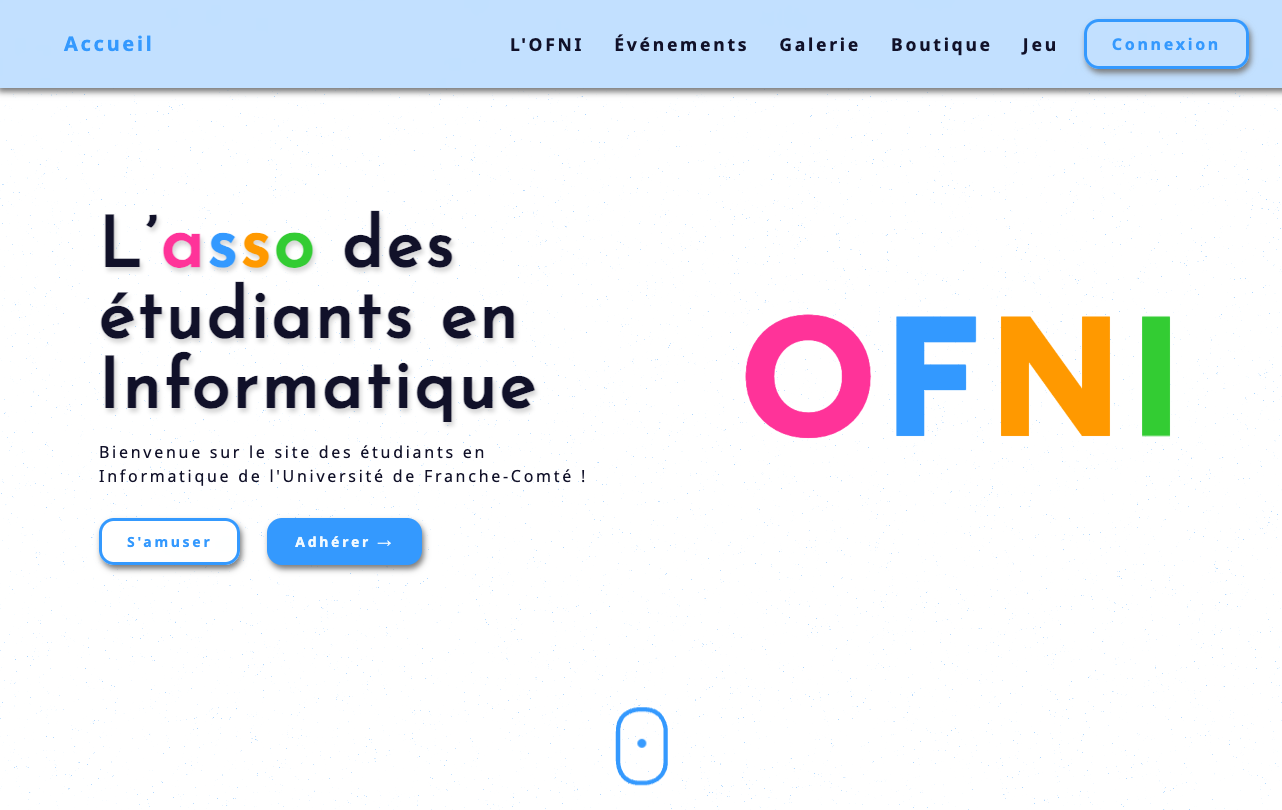
\includegraphics[width=8cm]{assets/pictures/home-page.png}
  \end{center}

  \vspace*{1cm}
  \noindent
  \large{\textbf{Tuteurs de projet:} \textsc{DEMOUGIN} Alexandre  et \textsc{PIERROT} Alicia}\\
  \vspace*{0.5cm}
  
  \noindent
  \large{\textbf{Établissement de formation:} \textsc{\univ}}\\

\end{titlepage}
\ClearShipoutPicture
\thispagestyle{empty}
\setcounter{page}{0}
\null
\newpage
\chapter*{Remerciements}

Nous tenons tout d'abord à remercier nos tuteurs de projet pour leur soutien et leur encadrement, Monsieur \nom{Alexandre}{Demougin} et Madame \nom{Alicia}{Pierrot}, qui nous ont guidés tout au long de ce projet. 
Leurs précieuses indications et conseils ont été d'une grande aide pour la réalisation du projet.
\bigskip

Nous remercions également l'\univ, et plus particulièrement le département d'informatique, qui, de par ses enseignements, nous a transmis les savoirs et les compétences nécessaires à la réalisation de ce projet.
\bigskip

Enfin, nous remercions également les étudiants testeurs, qui nous ont fait part de leurs retours sur le site que nous avons produit.

\cleardoublepage
% \Large
\tableofcontents
\listoffigures
% \listofalgorithms
\normalsize
\chapter{Glossaire}
\label{chap:glossary}

\begin{description}
    \item[CMS] Un système de gestion de contenu (\langue{Content Management System}) est un logiciel qui permet de créer, modifier et publier du contenu sur un site \web.
    \item[CAS] Le \langue{Central Authentication Service} est un système d'authentification centralisé permettant à un utilisateur de se connecter à plusieurs services avec un seul identifiant.
    \item[RGPD] Le \citer{Règlement Général sur la Protection des Données} est un règlement de l'Union Européenne qui encadre le traitement des données personnelles.
    \item[Regex] Une expression régulière (\langue{Regular Expression}) est une chaîne de caractères qui décrit un ensemble de chaînes de caractères possibles selon une syntaxe précise.
\end{description}

\noindent\HRule
\vspace{1cm}

\Large\noindent \strong{Terminologie spécifique au site de l'\ofni}\normalsize

\begin{description}
    \item[Instance d'événement] Une occurrence d'un événement, c'est-à-dire une édition précise de ce dernier.
    \item[Form-Widget] Un ensemble de champs de formulaire qui peuvent être réutilisés pour créer des formulaires plus complexes. Il en existe trois types~: \code{natif}, \code{composite} et \code{liste}.
\end{description}

\chapter{Introduction}


\chapter{Le site web de l'association \ofni}
\label{chap:site}

Le but de ce projet est de réaliser le site internet de l'association \ofni.

\section{Le projet}

Ce rapport présente le développement que nous avons réalisé dans le cadre du projet tutoré de troisième année de Licence Informatique à l'\univ\ de \propre{Besançon}.
\bigskip

Le sujet de ce projet était de développer un site \web\ pour une association étudiante, en équipe de trois personnes. L'objectif était de mobiliser nos compétences en développement \web\ tout en en acquérant de nouvelles.

Pour cela, nous avons été encadrés par Monsieur \nom{Alexandre}{Demougin} et Madame \nom{Alicia}{Pierrot}, depuis la conception du site jusqu'à sa mise en ligne, ainsi que pour la rédaction de ce rapport et la préparation de notre soutenance orale.
\bigskip

Nous avions quelques mois pour mener à bien ce projet, qui était divisé en trois grandes phases:

La première, de novembre à décembre 2024, portait sur la phase de conception et de maquettage du site. 
Celle-ci consistait dans un premier temps à trouver les fonctionnalités du site ainsi que les besoins auxquels il devait répondre. 
Dans un second temps, cette phase consistait en l'élaboration de la maquette du site, contenant l'entièreté des pages du site ainsi que leurs visuels.

La seconde étape, de janvier à février, était la phase de développement du site. 
Celle-ci correspondait à une période de recherche et de réflexion sur les technologies existantes, le choix des plus adaptées pour la réalisation du projet, ainsi que le développement et le codage du site.

Enfin, la dernière phase, de février à mars, était la phase de réalisation de ce rapport et de la soutenance orale.

\section{L'association \ofni}

Fondée en 1997, l'\ofni\ est l'association des étudiants en informatique de l'\univ\ de \propre{Besançon}.
\bigskip

L'association a pour but de rassembler les étudiants des différentes promotions autour d'activités communes (sorties, barbecues, Nuit de l'Info, etc.) et de favoriser l'entraide entre promotions.

L'\ofni\ joue également un rôle d’intermédiaire entre ses membres, les chercheurs et les entreprises en maintenant un réseau d’anciens étudiants et des contacts avec ses sponsors.
\bigskip

Le projet restait lible sur le choix de l'association et des technologies utilisées.
C'est en équipe que nous avons choisi de réaliser le site de l'association \ofni{}. 
Notre équipe faisant partie du bureau actuel de l'association, notre choix s'est donc imposé naturellement. 
Bien que l'association avait déjà un site, celui-ci était obsolète et ne répondait plus aux besoins actuels de l'association, comme le montre la \figureref{oldsite}.
De plus, il n'était plus maintenu et présentait des failles de sécurité.
\bigskip

\begin{figure}[!ht]
    \centering% 
    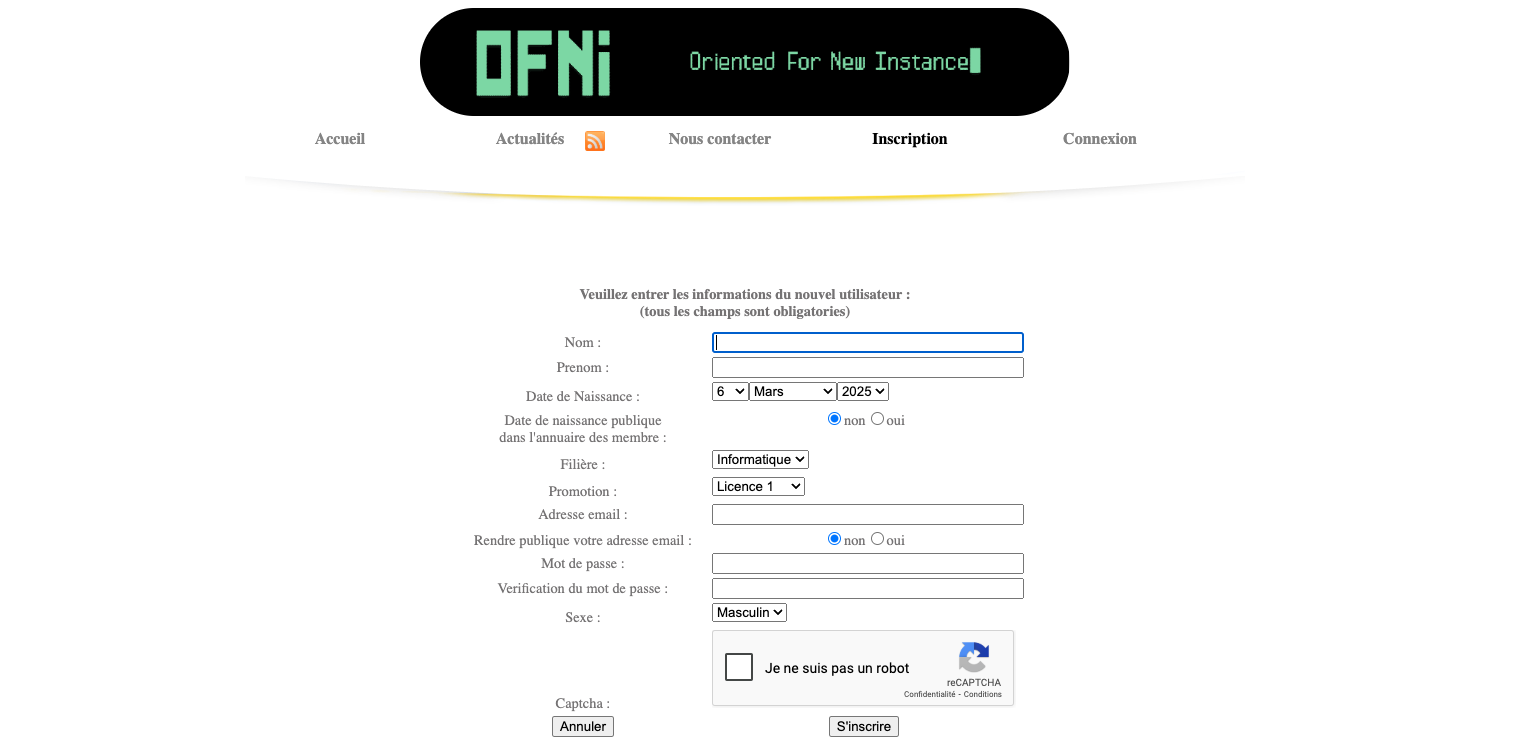
\includegraphics[width=15cm]{assets/pictures/old-site.png}
    \caption[\emph{Ancien site de l'association \ofni}]{Ancien site de l'association \ofni}%
    \label{oldsite}%
\end{figure}
\bigskip

Les consignes sur la réalisation du site étaient de créer une interface claire et intuitive, de développer une solution robuste et fonctionnelle, le tout en mettant l’accent sur l’efficacité et la maintenabilité du site.
\bigskip

Les fonctionnalités envisagées incluaient la présentation des activités de l’association, une vitrine pour les projets étudiants, la possibilité de réaliser des sondages pour les événements et la mise à disposition d’informations pour les lycéens souhaitant découvrir l’association.

\chapter{Le développement du nouveau site}

\section{La répartition du travail}
\section{Le maquettage du nouveau site}
\subsection{Version manuscrite}
\subsection{Version finale sur Figma}
\section{Les technologies utilisées}
\subsection{Le framework Symfony}
\subsection{...}
\section{Les difficultés rencontrées}


\chapter{Le travail réalisé}

\section{Ce qui a été implémenté}
\section{Ce qui n'a pas été implémenté}
\section{Projection pour l'avenir}


\section{Conclusion}
\sectitle{Conclusion}

\begin{frame}
    \frametitle{Conclusion}
    \centering
    \textbf{Bilan}: Première version fontionnelle du site, sécurisée, adaptée aux besoins de l’association
    \vspace{1cm}

    \textbf{Ajout}: jeu OFNIvaders
    \vspace{1cm}

    \textbf{Pistes d'améliorations}: CMS, calendrier interactif, SEO, etc.
\end{frame}

\begin{frame}[plain, noframenumbering]
    \scshape\huge\centering
    \vspace{1cm}
    Merci pour votre attention !\par
    \vspace{2cm}
    Avez-vous des questions ?\par
\end{frame}

% \appendix
\renewcommand{\thefigure}{\Alph{figure}}

\chapter*{Annexes}

\begin{figure}[H]
    \centering
    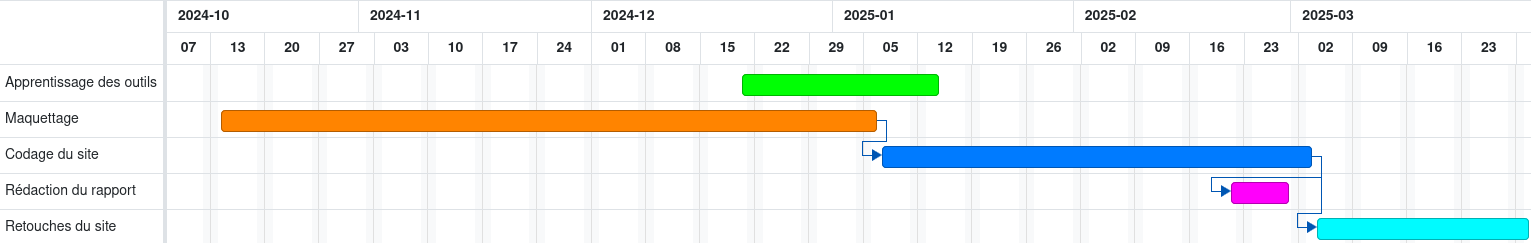
\includegraphics[width=\textwidth]{assets/pictures/gantt.png}
    \caption{Diagramme de Gantt du projet}
    \label{anx:gantt}
\end{figure}

\begin{figure}[H]
    \centering
    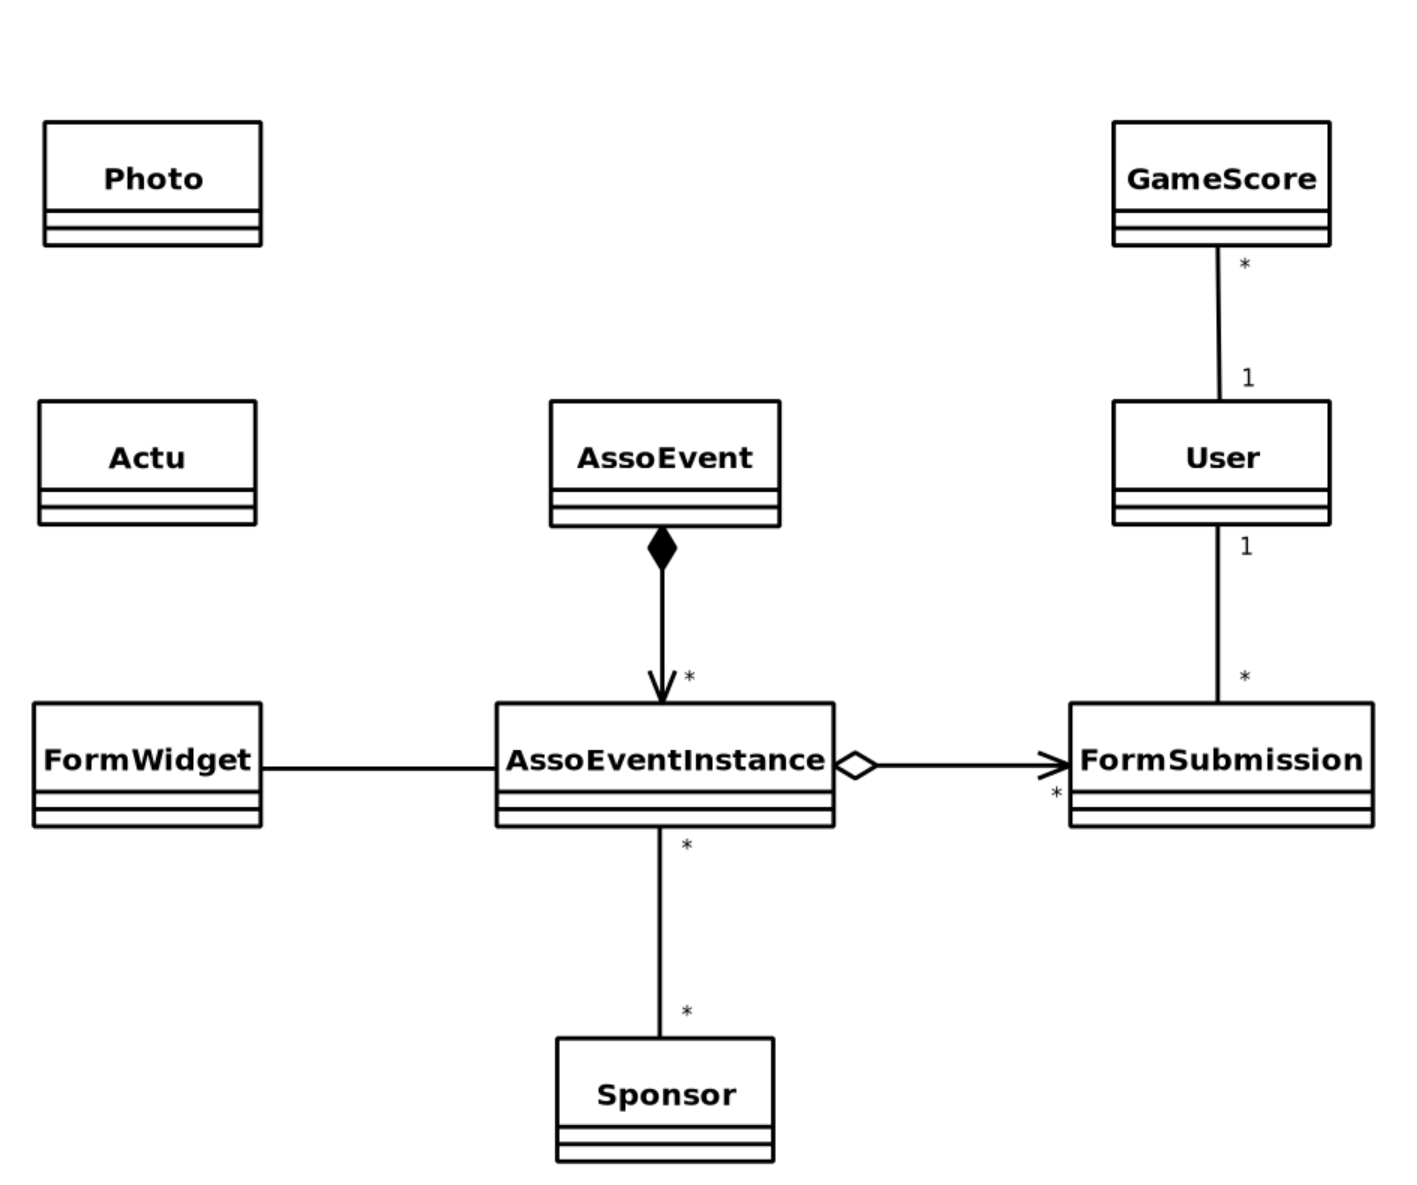
\includegraphics[width=\textwidth]{assets/pictures/database.png}
    \caption{Structure simplifiée de la base de donnée}
    \label{anx:gantt}
\end{figure}

\chapter{Bibliographie}

\begin{itemize}
    \item\bibquote{Symfony Documentation}{Symfony SAS}{https://symfony.com/doc/current/index.html}
    \item\bibquote{Twig Documentation}{Symfony SAS}{https://twig.symfony.com/doc/3.x/}
    \item\bibquote{Doctrine Documentation}{Doctrine Community}{https://www.doctrine-project.org/projects/doctrine-orm/en/2.9/index.html}
    \item\bibquote{PHP Documentation}{The PHP Group}{https://www.php.net/docs.php}
\end{itemize}


\end{document}
